\documentclass[12pt]{article}
\usepackage[utf8]{inputenc}
\usepackage[T1]{fontenc}
\usepackage[spanish]{babel}%caracteres en español
\usepackage{verbatim}
\title{\huge \textbf{\textsc{Evaluación 2}}}%titulo en grande-negritas-versalitas
\author{Álvarez Sánchez Francisco Eduardo}
\usepackage{graphicx}%para cargar imagenes
\usepackage{wrapfig} %para acomodar figuras y que compartan espacio con texto
\usepackage{fancyhdr}
\pagestyle{fancy}
\fancyhf{}
\usepackage{enumerate}
\usepackage{cite}
\usepackage{hyperref}
\usepackage{bookmark}
\fancyfoot[R]{Página \thepage}
\setlength\headheight{15 pt}
\fancyhead[L]{Francisco Eduardo Álvarez Sánchez}
\fancyhead[R]{Física Computacional I}
\usepackage{booktabs}
\usepackage[nottoc,numbib]{tocbibind}
\usepackage{dsfont}
\usepackage{hyperref}
\author{Álvarez Sánchez Francisco Eduardo}
\title{\textbf{\textsc{Actividad 8: Atractores extraños. Efecto mariposa}}} 
\date{\today}

\begin{document}

\begin{titlepage}
	\centering
    \begin{figure}[ht!]
    \centering
    \includegraphics[scale=0.5]{escudo.png}
    
    \textbf{UNIVERSIDAD DE SONORA \\ DIVISIÓN DE CIENCIAS EXACTAS Y NATURALES \\ DEPARTAMENTO DE FÍSICA \\ LICENCIATURA EN FÍSICA}
	\maketitle
    \hrule \bigskip
    \large{Física computacional I}\\
	Profr. Carlos Lizárraga Celaya
    \end{figure}
\thispagestyle{empty}
\end{titlepage}

\newpage

\section{Resumen}
\noindent En el siguiente trabajo se tuvo como principal objetivo el estudio del trabajo de Edward Lorentz, que se le presento cuando se encontraba estudiando la dinámica de la atmósfera y es un concepto de la teoría del caos.

Con la ayuda de matplotlib y lorenz\_attractor.py haremos la representación gráfica que le da nombre a este efecto gracias a su forma de mariposa o un ocho. 

\section{Síntesis}
\noindent El efecto mariposa es un concepto de a teoría del caos. La idea es que, dadas unas circunstancias peculiares de el tiempo y condiciones iniciales de un determinado sistema dinámico caótico, cualquier pequeña discrepancia entre dos situaciones conn una variación pequeña en los datos iniciales, cabe resaltar que sin duda alguna y sin explicación científica, acabará dando lugar a situaciones donde ambos sistemas evolucionan en ciertos aspectos de forma completamente diferente.

El pionero del desarrollo de la teoría de caos es el matemático y meteorólogo estadounidense Edward Norton Lorenz, quien fue el que introdujo el concepto de atractores extraños y acuñó el término mariposa. 

Lorenz construyó un modelo matemático muy simplificado, que intentaba capturar el comportamiento de la convección en la atmósfera. Al estudiar las soluciones de su modelo se dio cuenta que alteraciones mínimas en los valores de las variables iniciales resultaban en soluciones ampliamente divergentes.
\newpage
\section{Representación gráfica}
\noindent Para crear una representación gráfica del atractor de Lorentz se utilizó matplotlib junto con el código que describe las ecuaciones que representan la evolución de las variables espaciales $x$,$y$,$z$, dado los parámetros $\sigma$, $\beta$ y $\rho$, a través de la especificación de las derivadas de tiempo de las variables espaciales:

$${\rm d}x/{\rm d}t=\sigma(y-x)$$

$${\rm d}y/{\rm d}t=x(\rho-z)$$

$${\rm d}z/{\rm d}t=xy-\beta z$$

En la siguiente sección de código tenemos los pandas necesarios y las variables correspondientes para realizar la primera gráfica, que es la que representara a este efecto. En esta parte basicamente ponemos las condiciones iniciales y damos los parámetros de las gráficas. 

\begin{verbatim}
import numpy as np

import matplotlib.pyplot as plt

from mpl_toolkits.mplot3d import Axes3D

def lorenz(x, y, z, s=10, r=28, b=2.667):
    x_dot = s*(y - x)
    y_dot = r*x - y - x*z
    z_dot = x*y - b*z
    return x_dot, y_dot, z_dot
    

dt = 0.01
stepCnt = 10000
xs = np.empty((stepCnt + 1,))
ys = np.empty((stepCnt + 1,))
zs = np.empty((stepCnt + 1,))

xs[0], ys[0], zs[0] = (0., 1., 1.05)

for i in range(stepCnt):
    x_dot, y_dot, z_dot = lorenz(xs[i], ys[i], zs[i])
    xs[i + 1] = xs[i] + (x_dot * dt)
    ys[i + 1] = ys[i] + (y_dot * dt)
    zs[i + 1] = zs[i] + (z_dot * dt)
fig = plt.figure()
ax = fig.gca(projection='3d')
ax.plot(xs, ys, zs, lw=0.5,color="b")
ax.set_xlabel("Eje X ")
ax.set_ylabel("Eje Y ")
ax.set_zlabel("Eje Z ")
ax.set_title("Atractor de Lorentz")

plt.show()

\end{verbatim}
 El resultado que no dará esta sección de código sera la siguiente gráfica
 
 \begin{figure}[ht!]
 \centering
 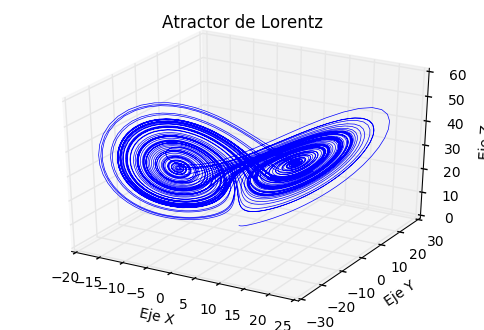
\includegraphics[scale=0.5]{1.png}
 \end{figure}
 
 Ahora, para realizar el video utilizamos el siguiente código en el cual se especifican los parámetros del video, etc.
 
 \begin{verbatim}
 import numpy as np
from scipy import integrate

from matplotlib import pyplot as plt
from mpl_toolkits.mplot3d import Axes3D
from matplotlib.colors import cnames
from matplotlib import animation

N_trajectories = 30


def lorentz_deriv(params, t0, sigma=10., beta=8./3, rho=28.0):
    """Compute the time-derivative of a Lorentz system."""
    x, y, z = params
    return [sigma * (y - x), x * (rho - z) - y, x * y - beta * z]


# Choose random starting points, uniformly distributed from -15 to 15
np.random.seed(1)
x0 = -15 + 30 * np.random.random((N_trajectories, 3))

# Solve for the trajectories
t = np.linspace(0, 4, 1000)
x_t = np.asarray([integrate.odeint(lorentz_deriv, x0i, t)
                  for x0i in x0])

# Set up figure & 3D axis for animation
fig = plt.figure()
ax = fig.add_axes([0, 0, 1, 1], projection='3d')
ax.axis('on')

# choose a different color for each trajectory
colors = plt.cm.jet(np.linspace(0, 1, N_trajectories))

# set up lines and points
lines = [ax.plot([], [], [], '-', c=c)[0]
for c in colors]
pts = [ax.plot([], [], [], 'o', c=c)[0]
for c in colors]

# prepare the axes limits
ax.set_xlim((-25, 25))
ax.set_ylim((-35, 35))
ax.set_zlim((5, 55))

# set point-of-view: specified by (altitude degrees, azimuth degrees)
ax.view_init(30, 0)

# initialization function: plot the background of each frame
def init():
    for line, pt in zip(lines, pts):
        line.set_data([], [])
        line.set_3d_properties([])

        pt.set_data([], [])
        pt.set_3d_properties([])
    return lines + pts

# animation function.  This will be called sequentially with the frame number
def animate(i):
    # we'll step two time-steps per frame.  This leads to nice results.
    i = (2 * i) % x_t.shape[1]

    for line, pt, xi in zip(lines, pts, x_t):
        x, y, z = xi[:i].T
        line.set_data(x, y)
        line.set_3d_properties(z)

        pt.set_data(x[-1:], y[-1:])
        pt.set_3d_properties(z[-1:])

    ax.view_init(30, 0.3 * i)
    fig.canvas.draw()
    return lines + pts

# instantiate the animator.
anim = animation.FuncAnimation(fig, animate, init_func=init,
                               frames=500, interval=30, blit=True)

# Save as mp4. This requires mplayer or ffmpeg to be installed
anim.save('Atractor de Lorentz.mp4', fps=15, extra_args=['-vcodec', 'libx264'])

plt.show()

 \end{verbatim}

El resultado será un video y aparte Python da la siguiente imagen. 
\begin{figure}[ht!]
\centering
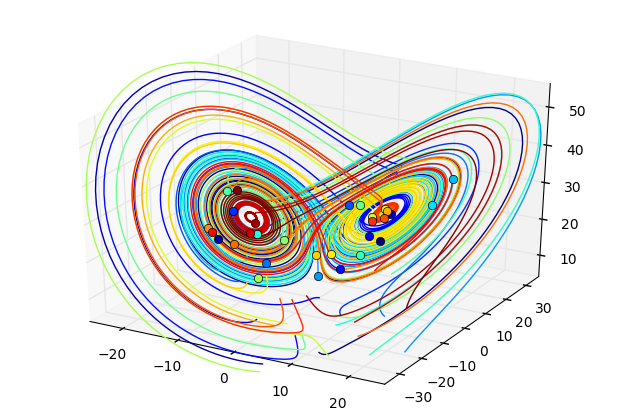
\includegraphics[scale=0.75]{2.png}
\end{figure}

\begin{thebibliography}{X}
\bibitem{FC} \textsc{Carlos Lizárraga Celaya},
\textit{Fisica computacional I }, Actividad 8,
Atractores extraños. El efecto mariposa. http://computacional1.pbworks.com/w/page/117689967/Actividad\%208\%20(2017-1) (Consultado el 15 de Mayo de 2017)
\bibitem{Dan} \textsc{Pythonic perambulations.},
\textit{Solving the Lorenz System}https://jakevdp.github.io/blog/2013/02/16/animating-the-lorentz-system-in-3d/ (Consultado el 15 de Mayo de 2017)
\end{thebibliography}



\end{document}
